\documentclass[]{article}
\usepackage{graphicx}
\usepackage{float}
\usepackage[english]{babel}
\usepackage{titlepic}
\usepackage{hyperref}
\usepackage{float}
\usepackage{multirow}
\usepackage{floatflt}
\usepackage[style=authoryear-ibid,backend=bibtex]{biblatex}
\hypersetup{
	citecolor=black,
	urlbordercolor={1 1 1},
	colorlinks=true,
	linkcolor=blue,
	filecolor=blue,      
	urlcolor=blue,
}
\addbibresource{test.bib}
\begin{document}
	\begin{titlepage}
		\centering
		\title{Inscriber}
		\author{by Christoffer Lundström}
		\date{\centering
			July 21, 2019\endgraf\vspace{2cm}\endgraf
			Development of Mobile Applications - 5DV209\endgraf
			Examinator: Johan Eliasson\endgraf
			}
		\titlepic{
\includegraphics[width = 40mm]{logo.png}}	
		\maketitle
		\thispagestyle{empty}
	\end{titlepage}
	\newpage
	\tableofcontents
	\thispagestyle{empty}
	\newpage
	
\begin{flushleft}
\section{Introduction}


\subsection{General information}

\begin{figure}[H]
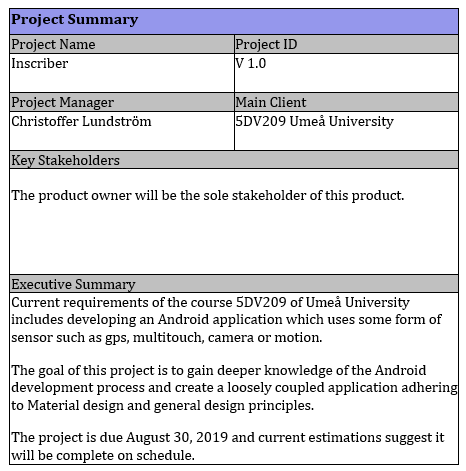
\includegraphics[scale=0.9]{summary.png}
\end{figure}

\newpage
\subsection{Vision}

My vision for this project is to create an application inspired by geolocation and the phenomenon of geocaching. Similar to applications such as Pokemon GO and Geocaching\texttrademark. It will be a simple but stable cloud based application where the user is able to drop short text-based notes at places they come across. The user can later look back on these locations and notes in a list together with a map and marker of the location. These notes will be called Inscriptions, like the mark you leave on a tree.\medskip

Future versions of the application could include the ability to share these Inscriptions with friends or even to the public by notifying those who come across the area you Inscribed. The ability to make time-based Inscriptions is also a worthy addition. These additions are the main reasoning behind choosing a cloud based database for the project.\medskip

\subsubsection{Target audience}
This app will be primarily suitable for explorers, hikers or outgoing people but usable by anyone. The application could serve as a reminder of a great mushroom spot, or to mark the start of a hiking trail. Any spot worthy of remembrance is worth an Inscription.

\subsubsection{Play store description}

Venture into the wild and leave your mark.
Leave customized messages for the next traveller.
Get notified when near an Inscription.

\subsubsection{Grade}
I aim for the higher grade, VG or A.
\newpage

\section{Project plan}

This will be the main project plan for the Android application. The project will be written in Java 1.8 using Android Studio v3.5.0 and GitHub for version control.

The main approach of this project is to use an agile development method to reduce the amount of documentation. It will use Google Firebase for cloud services.

\subsection{Justification}

This product will fill a spot as a map-based notebook which could be used for multiple purposes.
The application is also a requirement of 5DV209.

\subsection{Stakeholders}
The project manager(Christoffer Lundström) is the sole stakeholder.

\subsection{Resources}
This project will require at least 80 hours of work. Some of this time will be used for research. The project manager will be the only resource available.

\subsection{Hard- and Software Requirements}
The application is developed for Android API 19-28 and thus requires a device running Android.
Furthermore the application is projected to reserve around 60-100mb of ram on the device making it viable for most phones or tablets. The app is cloud based and requires an internet connection.\medskip

The application uses a few external libraries such as SDP\parencite{sdp} and SSP\parencite{ssp} which are extensions to the DP and SP system of Android. They scale text and ui elements automatically for most devices which reduces time spent on porting UI for different screen-sizes.\medskip

Furthermore Glide\parencite{glide:1} and AndroidImageSlider\parencite{slider:1} are used for smooth image-transitions in the app guide.

\subsection{Scope, Constraints and Assumptions}

The scope of this project will be limited by a strict deadline, 30th of August. This will be a limiting factor to the development of features for the application. The scope will most likely cover basic features of the application such as creating an Inscription, viewing these together with map previews of each location.\smallskip

Assuming the current vision is feasible for development the features of this application should be implemented on schedule.



\section{Risk analysis}

\subsection{List of risks}

\begin{figure}[H]
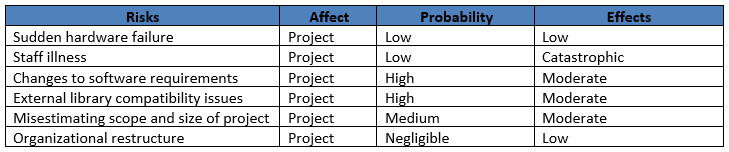
\includegraphics[scale=0.8]{risks.png}
\end{figure}


\subsection{Risk strategy}
The first step to avoid any project risks is to use GitHub for version control. This should mitigate any sudden hardware failures. Misestimating the scale and difficulty of the features proposed in the vision is always a risk for small projects, this should be no exception.\medskip 

Another strategy to avoid missing the deadline is to have the project complete by 20th of August to leave 10 days for any unforeseen events or difficulties with the project.\medskip

Changes to the software requirements is a huge risk and it is quite unavoidable due to limited experience of Android development. This is mitigated by being careful with the amount of implemented features for version 1.0. It is a safer approach to make sure a few are well functioning and thoroughly tested before release as most users only give the application one chance. This allows for a controlled rollout of updates moving forward.

\subsection{Contingency and monitoring}
Should the project fail to deliver on schedule there are extended deadlines to work towards, the last one being 7th of October. This project uses a few external libraries and these will be closely monitored during the development process. It is essential that no updates are pushed to the project without proper software validation and verification. Because these libraries are open source the risk of forced updates are non-existent and can be safely used.
\newpage
\section{Requirements Analysis}
\subsection{Functional}

This section will cover some important use cases of the application.\newline

\noindent\fbox{%
	\parbox{10cm}{%
		\begin{center}
			Use-Case - Inscribe
		\end{center}
		
		Pre-condition: None.\newline
		Post-condition: POST call to cloud.\newline
		
		Main Scenario:\newline
		1. User wants to Inscribe a location.\newline
		2. User clicks Inscribe button.\newline
		3. Add Inscription dialog is opened.\newline
		4. User writes a memo/note.\newline
		5. User presses Add.\newline
		6. Inscription is added to \textit{Your Inscriptions} view.\newline
		7. Marker is added to main map.\newline
		
		Alternative Scenario:\newline
		5. User presses back or cancel.\newline
	}
}\medskip

\noindent\fbox{%
	\parbox{10cm}{%
		\begin{center}
			Use-Case - View guide
		\end{center}
		
		Pre-condition: Guide dialog is present.\newline
		Post-condition: Activity and DialogFragment destroyed.\newline
		
		Main Scenario:\newline
		1. User wants to know how the application works.\newline
		2. User clicks \textit{SHOW ME}.\newline
		3. Guide Activity is started.\newline
		4. User scrolls through infommercial images.\newline
		5. User clicks button \textit{GOT IT}.\newline
		6. Activity is closed.\newline
		
		Alternative Scenario:\newline
		2. User clicks Hide.\newline
		5. User clicks back.
	}
}\medskip

\noindent\fbox{%
	\parbox{10cm}{%
		\begin{center}
			Use-Case - Reset data
		\end{center}
		
		Pre-condition: User has opened the Settings view.\newline
		Post-condition: DELETE call to Cloud.\newline
		
		Main Scenario:\newline
		1. User wants to reset Inscriptions.\newline
		2. User clicks preference \textit{Reset data}.\newline
		3. Confirmation dialog is opened.\newline
		4. User accepts reset.\newline
		5. User is returned to Settings view.\newline
		
		Alternative Scenario:\newline
		3. User clicks Cancel and aborts action.\newline
		5. User clicks back.\newline
	}
}\medskip

\noindent\fbox{%
	\parbox{10cm}{%
		\begin{center}
			Use-Case - View Inscriptions
		\end{center}
		
		Pre-condition: User has started the application.\newline
		Post-condition: None.\newline
		
		Main Scenario:\newline
		1. User wants to view Inscriptions.\newline
		2. User switches to \textit{Your Inscriptions}-tab.\newline
		3. Recycler-view is displayed with a list of Inscriptions.\newline
		4. User pinches the map preview for a closer view of location.\newline
		
	}
}\medskip

\noindent\fbox{%
	\parbox{10cm}{%
		\begin{center}
			Use-Case - Send feedback
		\end{center}
		
		Pre-condition: User has opened the Settings view.\newline
		Post-condition: None.\newline
		
		Main Scenario:\newline
		1. User wants to send the developer feedback.\newline
		2. User clicks Send feedback preference.\newline
		3. User is offered a predefined email template with an email-app of personal choice.\newline
		
		Alternative Scenario:\newline
		3. User clicks back or cancel.\newline
		
		
	}
}\medskip


\subsection{Non-Functional}

This section will cover requirements related to performance, accessibility, stability, ethics and safety.\newline

\subsubsection{Performance}

The project's current state includes only the essential features. Performance should therefore reflect this. Because the application requires an internet connection it is very important that the data-packets are light. This is one of the few ways to influence app latency other than recommending a fast connection.\medskip

Another important feature of the application is to have private Inscriptions available even in offline conditions. In future updates a local copy of the collection could be stored on the device which is synced to the cloud when a connection is available.\medskip

To make the app light-weight and smooth it is important to use scalable solutions such as Recycler-views and frame-layouts which reduces the need of allocated memory.

\subsubsection{Privacy, ethics \& security}

User privacy and security is an important focus of the application. Therefore only a few values which could be considered private should be collected. To identify each user a unique application id (firebase instance id) is produced. It is used for retrieving and posting new \textit{Inscriptions} to the cloud.\smallskip

By choosing this identifier the need for keeping another user reference such as email or login name is avoided. This approach requires no authentication and carries less overhead than firebase authentication but is more fragile to changes because each identifier is bound to the app installation. Reinstallation, clearing of app-cache or restoration of a backup will change the identifier and separate the user from its Inscriptions.\medskip

User locations stored together with private messages in Inscriptions can be very intrusive for privacy. Therefore the data is to be separated from any details which could identify a user. The collected data should also be transferred to firebase over a secure connection (HTTPS)\parencite{deception}. 

\begin{figure}[H]
	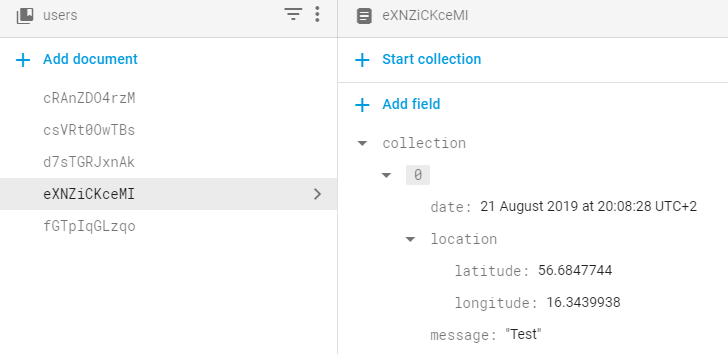
\includegraphics[width=\linewidth, height=60mm]{leak.png}
	\caption{Anonymous Inscription database entries.}
	\label{fig:anon_entries}
\end{figure}


In case of a complete data-leak no user should have to worry about being identified. From a security perspective end-users are the final variable to rely on. It should be clear in the application policy that no sensitive information should be posted in the message field of the Inscription and the users should be well-informed. This is likely the greatest privacy and security risk of all.\medskip

The ethical dilemma of collecting user data is an incongruous topic. The risks of keeping anonymity and privacy for users is of course that the service is used illegally or maliciously. Developers have an obligation to maintain confidentiality not only to their subject platform, but to the states in which the app is used.\medskip

In version 1.0 Inscriptions are private by default and does not include the ability to share Inscriptions publicly which avoids some of the risks previously mentioned, which also is recommended by Googles policy center\parencite{enforcement}.
 However, in future updates there should be robust continuous monitoring of public user generated content (Inscriptions) and sampling of data to discover malicious activity and to make sure no policies are breached. One such monitoring system could include manual or automatic scanning of content and a report feature with which the community self-moderates\parencite{usergen}.\medskip

Future plans include encryption of private Inscriptions for another layer of privacy for the user, but also to keep public Inscriptions unencrypted for monitoring purposes.

\newpage

\section {Design}

The app is designed to have instantaneous access to its core features. A simple swipe or press of a tab will be enough to switch between the main views. Two of those main features are the map view and the inscription view.\medskip

The first design choice was to create a main activity which sets up a toolbar, fragment-container and a tab-manager.\medskip

This section will cover some of the fragments used in the application. All these views are also designed with landscape compatibility.

\subsection{Map Fragment}

\begin{floatingfigure}[r]{0.3\linewidth}
	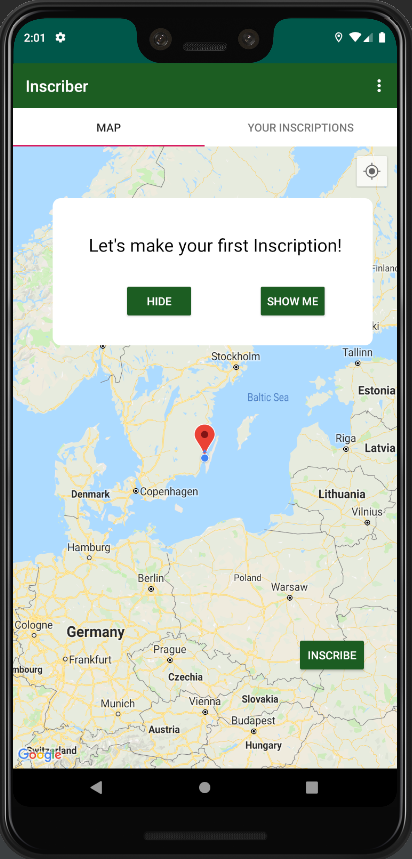
\includegraphics[scale=0.4]{mapfrag.png}
	\caption{The fragment contains a map, button and dialog.}
	\label{fig:map}
	\vspace{\dimexpr0.3\baselineskip-\topskip}
\end{floatingfigure}
\medskip
This fragment is created in the main container at start. It implements a Google map which is used to find a user's location and look around the general area for Inscribed locations. It also handles permission requests, creation of a guide dialog and an \textit{Add Inscription} button which follows a general green theme of the app and is compliant with \textit{material design}\parencite{buttons}. It is placed at an easily reached location of the screen.\medskip

The guide dialog is either dismissed or used to start a new guide activity intended to guide the user through the application.\medskip

The add inscription dialog opens a simple \textit{EditText} dialog in which the user can add notes to the current location. This dialog creates a new instance of an Inscription object which is returned to the map fragment, added to the users collection and a \textit{POST} request is sent to the cloud via use of the \textit{InscriptionService}.

\newpage
\left\subsection{Inscription-list Fragment}

\begin{floatingfigure}[r]{0.3\linewidth}
	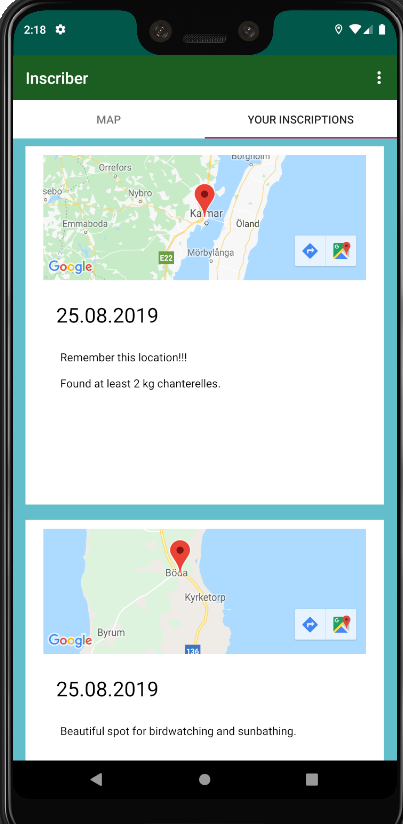
\includegraphics[scale=0.4]{inscription.png}
	\caption{Two inscriptions are shown in the recycler-view.}
	\label{fig:inscription}
	\vspace{\dimexpr0.3\baselineskip-\topskip}
\end{floatingfigure}
\medskip
This fragment contains a recycler-view responsible for displaying Inscriptions and keeping the list of Inscriptions synced with firebase. It does this by using the custom class \textit{InscriptionService} to attach a firestore \textit{snapshot-listener} on the users database-entry which acts as a webhook and immediately sends any updates to its listeners.\medskip


A Google \textit{lite-map} is also used for each location. It is a tiny interactive map with a marker of the Inscription location\parencite{lite}.\medskip


Currently there are no limitations on the amount of Inscriptions in the list, or on the frequency of Inscriptions saved. This must be addressed prior to a public release to avoid spam or expensive traffic fees.
\newpage

\left\subsection{Settings Fragment}

\begin{floatingfigure}[r]{0.3\linewidth}
	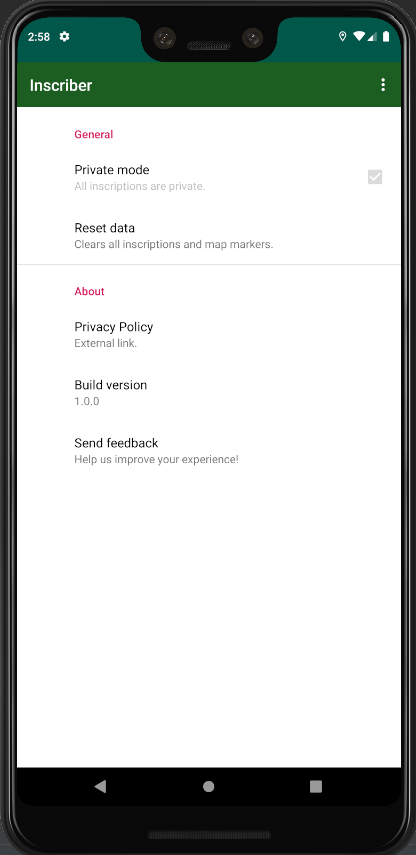
\includegraphics[scale=0.4]{settings.png}
	\caption{The settings view.}
	\label{fig:settings}
	\vspace{\dimexpr0.3\baselineskip-\topskip}
\end{floatingfigure}
\medskip
This fragment is opened from the toolbar button and displayed in the main fragment container. It is important that the fragment is a singleton to prevent duplicate actions, therefore each press of the settings button checks for duplicates of the instance in the fragment-manager.\medskip

As of version 1.0 all Inscriptions are private and the the only actions available in the fragment are \textit{Reset Data} and \textit{Send feedback}.\medskip

Reset Data uses \textit{InscriptionService} to communicate with firebase and reset the users collection. This does not reset the firebase instance id to avoid unnecessary document creation in firestore cloud.\medskip

Send feedback is designed to start an email activity with pre-filled subject and email sender fields for easy communications with the developers.

\newpage
\left\subsection{Diagrams}

\begin{figure}[H]
	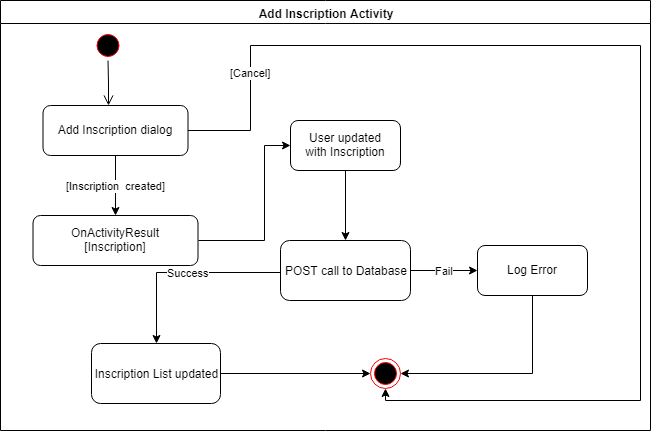
\includegraphics[width=\linewidth, height=70mm]{add_ins.png}
	\caption{Activity flow of adding an Inscription.}
	\label{fig:add_activity}
\end{figure}

\begin{figure}[H]
	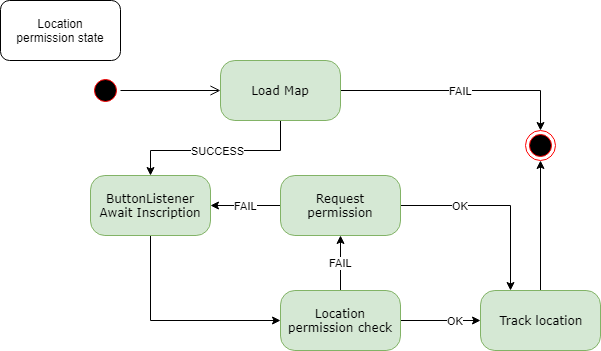
\includegraphics[width=\linewidth, height=50mm]{perm.png}
	\caption{Location state machine.}
	\label{fig:permission_state}
\end{figure}
\newpage

\left\subsection{Reflection}

The design of this app is fairly straightforward with a main fragment-container which is used as a placeholder for fragments added, removed or replaced by the fragment-manager. This approach is more dynamic and flexible rather than using different activities or hard-coded fragments. In that regard the app is designed with scalability in mind, and in preparation for future updates.\medskip

In early development each component implemented its own CRUD operations to the database. This turned out to be a bad approach which tightly coupled the components and made it hard to keep track of which object was most recently updated. This was later centralized to a single service managing all database-operations which facilitated communications.\medskip

During development the UI colour schemes and design templates changed at least a few times. The colour scheme is inspired by the green contrast of nature and the blue sky surrounding it. The scheme seemed fitting for an app targeted to explorers and hikers.\medskip

The choice of a cloud based backend for the app seemed like a necessity from the start. Had I begun using a local database it would most likely be difficult to migrate existing user data to the cloud in future updates.\medskip

I feel that the app almost is ready for a first release, however some additions would have to be made prior. Some of these are limiting of rate for Inscriptions, writing an app policy, unit testing with edge cases and saving of state when hiding the guide dialog.\medskip

To summarize I feel that the app development has been a tough, but worthwhile learning experience, and I feel very satisfied with the end results.

\newpage
\section{Test plan}

During development the app has undergone a bare minimum of testing. Most of the tests have been manual, which are prone to errors. Because of this, and lack of time for writing unit tests an automated apk analyser from firebase has been used.

\begin{figure}[H]
	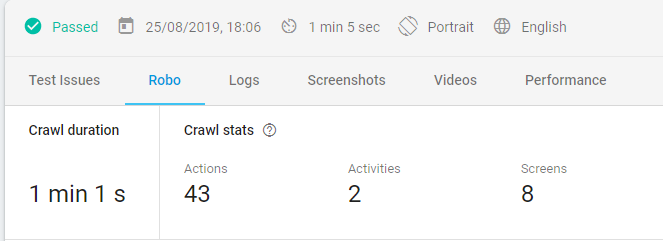
\includegraphics[width=\linewidth]{test1.png}
	\caption{Firebase test lab results.}
	\label{fig:test1}
\end{figure}

\begin{figure}[H]
	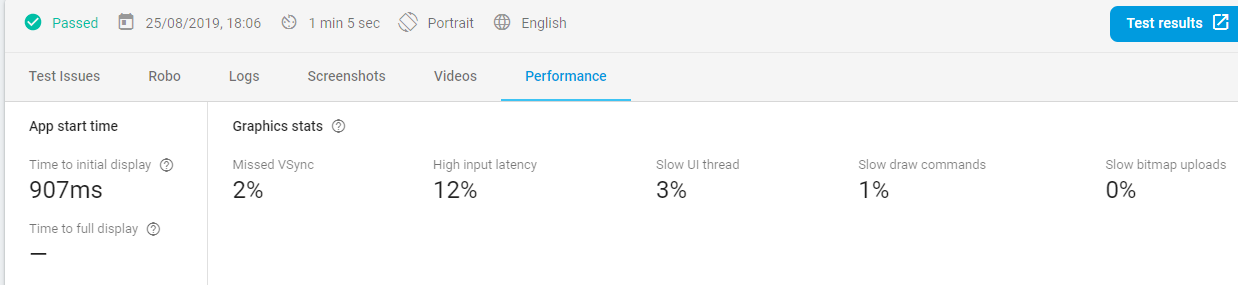
\includegraphics[width=\linewidth]{test2.png}
	\caption{Startup times and latency.}
	\label{fig:test2}
\end{figure}

\begin{figure}[H]
	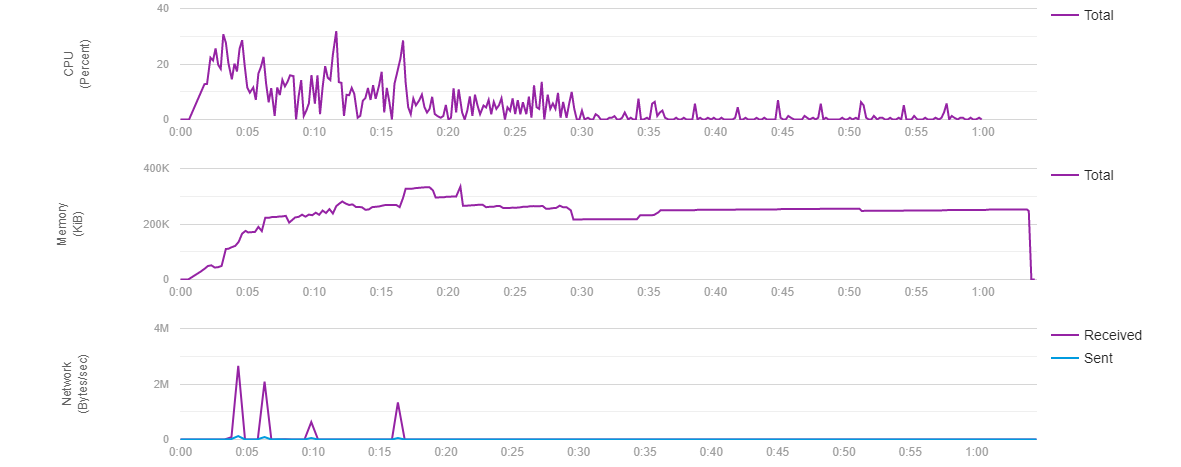
\includegraphics[width=\linewidth]{test3.png}
	\caption{Performance graph.}
	\label{fig:test3}
\end{figure}



\section{References}
\printbibliography[title={Online sources}]
\end{flushleft}
\end{document}          
